\documentclass{article}
\usepackage{amsmath}  % For math symbols
\usepackage{array}
\usepackage{graphicx} % Required for inserting images
\usepackage{lipsum}   % For dummy text, you can remove this if unnecessary
\usepackage{hyperref} % Include the hyperref package


\title{

\includegraphics[width=0.5\textwidth]{ist-logo.jpg}\\[1ex] % Image at the top, adjust width if needed
Machine Learning Report \\ 
\large Homework IV - Clustering and PCA
}
\author{ist1114964 - Axel Carapinha \\ ist1106565 - Martim Gordino}
\date{\today}

\begin{document}

\maketitle
\tableofcontents
\newpage

\section{Clustering}
\subsection{Exercise a)}

Firstly, by analysing the given information, we already know that:

\[
x_1 = \begin{pmatrix} 1 \\ 1 \end{pmatrix} , x_2 = \begin{pmatrix} -1 \\ -1 \end{pmatrix} , x_3 = \begin{pmatrix} 0.5 \\ 0.55 \end{pmatrix}
\]

\[
P(x \mid C = 1) = N\left(\mu^1 = \begin{pmatrix} 1 \\ 1 \end{pmatrix}, \quad \Sigma_1 = \begin{pmatrix} 1 & 0 \\ 0 & 1 \end{pmatrix}\right)
\]
\[
P(x \mid C = 2) = N\left(\mu^2 = \begin{pmatrix} -1 \\ -1 \end{pmatrix}, \quad \Sigma_2 = \begin{pmatrix} 1 & 0 \\ 0 & 1 \end{pmatrix}\right)
\]

We also know the prior probabilities of C:
\[
P(C = 1) = 0.6
\]
\[
P(C = 2) = 0.4
\]
\newline
Now, let´s calculate the likelihood and the joint probability for both clusters

\begin{itemize}

 \item[\textbullet] For \( x^{(1)} \), C = 1:
 
\[
\text{Likelihood: } p \left( x^{(1)} \mid C = 1 \right) = \frac{1}{2\pi} \frac{1}{\det(\Sigma_1)} \exp \left( -\frac{1}{2} \left( x^{(1)} - \mu^1 \right)^T \Sigma_1^{-1} \left( x^{(1)} - \mu^1 \right) \right)
\]

\[
= \frac{1}{2\pi} \frac{1}{1} \exp \left( -\frac{1}{2} \begin{pmatrix} 0 \\ 0 \end{pmatrix}^T \begin{pmatrix} 1 & 0 \\ 0 & 1 \end{pmatrix} \begin{pmatrix} 0 \\ 0 \end{pmatrix} \right)
\]

\[
= \frac{1}{2\pi} \exp \left( -\frac{1}{2} \cdot 0 \right) 
\]

\[
= \frac{1}{2\pi} \exp(0) = \frac{1}{2\pi}
\]

\[
\text{Joint Probability: } p(C = 1, x^{(1)}) = p(C = 1) \cdot p(x^{(1)} \mid C = 1) = 0.6 \times \frac{1}{2\pi} = 0.095
\]
\newpage

 \item[\textbullet] For \( x^{(1)} \), C = 2: 
 
\[
\text{Likelihood: } p \left( x^{(1)} \mid C = 2 \right) = \frac{1}{2\pi} \frac{1}{\det(\Sigma_2)} \exp \left( -\frac{1}{2} \left( x^{(1)} - \mu^2 \right)^T \Sigma_2^{-1} \left( x^{(1)} - \mu^2 \right) \right)
\]

\[
= \frac{1}{2\pi} \frac{1}{1} \exp \left( -\frac{1}{2} \begin{pmatrix} 2 \\ 2 \end{pmatrix}^T \begin{pmatrix} 1 & 0 \\ 0 & 1 \end{pmatrix} \begin{pmatrix} 2 \\ 2 \end{pmatrix} \right)
\]

\[
= \frac{1}{2\pi} \exp \left( -\frac{1}{2} \cdot 8 \right) 
\]

\[
= \frac{1}{2\pi} \exp(-4) = 0.003
\]

\[
\text{Joint Probability: } p(C = 2, x^{(1)}) = p(C = 2) \cdot p(x^{(1)} \mid C = 2) = 0.4 \times 0.003 = 0.0012
\]

Now, we can normalize both joint probabilities:

C = 1:
\[
p(C = 1 \mid x^{(1)}) = \frac{p(C = 1, x^{(1)})}{p(C = 1, x^{(1)}) + p(C = 2, x^{(1)})} = \frac{0.095}{0.095 + 0.0012} = 0.9875
\]

C = 2:
\[
p(C = 2 \mid x^{(1)}) = \frac{p(C = 2, x^{(1)})}{p(C = 1, x^{(1)}) + p(C = 2, x^{(1)})} = \frac{0.0012}{0.095 + 0.0012} = 0.0125
\]

 \item[\textbullet] For \( x^{(2)} \), C = 1: 

\[
\text{Likelihood: } p \left( x^{(2)} \mid C = 1 \right) = \frac{1}{2\pi} \frac{1}{\det(\Sigma_1)} \exp \left( -\frac{1}{2} \left( x^{(2)} - \mu^1 \right)^T \Sigma_1^{-1} \left( x^{(2)} - \mu^1 \right) \right)
\]

\[
= \frac{1}{2\pi} \frac{1}{1} \exp \left( -\frac{1}{2} \begin{pmatrix} -2 \\ -2 \end{pmatrix}^T \begin{pmatrix} 1 & 0 \\ 0 & 1 \end{pmatrix} \begin{pmatrix} -2 \\ -2 \end{pmatrix} \right)
\]

\[
= \frac{1}{2\pi} \exp \left( -\frac{1}{2} \cdot 8 \right) 
\]

\[
= \frac{1}{2\pi} \exp(-4) = 0.003
\]

\[
\text{Joint Probability: } p(C = 1, x^{(2)}) = p(C = 1) \cdot p(x^{(2)} \mid C = 1) = 0.6 \times 0.003 = 0.0018
\]

\newpage

 \item[\textbullet] For \( x^{(2)} \), C = 2: 

\[
\text{Likelihood: } p \left( x^{(2)} \mid C = 2 \right) = \frac{1}{2\pi} \frac{1}{\det(\Sigma_2)} \exp \left( -\frac{1}{2} \left( x^{(2)} - \mu^2 \right)^T \Sigma_2^{-1} \left( x^{(2)} - \mu^2 \right) \right)
\]

\[
= \frac{1}{2\pi} \frac{1}{1} \exp \left( -\frac{1}{2} \begin{pmatrix} 0 \\ 0 \end{pmatrix}^T \begin{pmatrix} 1 & 0 \\ 0 & 1 \end{pmatrix} \begin{pmatrix} 0 \\ 0 \end{pmatrix} \right)
\]

\[
= \frac{1}{2\pi} \exp \left( -\frac{1}{2} \cdot 0 \right) 
\]

\[
= \frac{1}{2\pi} \exp(0) = \frac{1}{2\pi}
\]

\[
\text{Joint Probability: } p(C = 2, x^{(2)}) = p(C = 2) \cdot p(x^{(2)} \mid C = 2) = 0.4 \times \frac{1}{2\pi} = 0.0637
\]

Again we normalize both joint probabilities:

C = 1:
\[
p(C = 1 \mid x^{(2)}) = \frac{p(C = 1, x^{(2)})}{p(C = 1, x^{(2)}) + p(C = 2, x^{(2)})} = \frac{0.0018}{0.0637 + 0.0018} = 0.0275
\]

C = 2:
\[
p(C = 1 \mid x^{(2)}) = \frac{p(C = 1, x^{(2)})}{p(C = 1, x^{(2)}) + p(C = 2, x^{(2)})} = \frac{0.0637}{0.0637 + 0.0018} = 0.9725
\]

 \item[\textbullet] For \( x^{(3)} \), C = 1: 

\[
\text{Likelihood: } p \left( x^{(3)} \mid C = 1 \right) = \frac{1}{2\pi} \frac{1}{\det(\Sigma_1)} \exp \left( -\frac{1}{2} \left( x^{3} - \mu^1 \right)^T \Sigma_1^{-1} \left( x^{(3)} - \mu^1 \right) \right)
\]

\[
= \frac{1}{2\pi} \frac{1}{1} \exp \left( -\frac{1}{2} \begin{pmatrix} -0.5 \\ -0.45 \end{pmatrix}^T \begin{pmatrix} 1 & 0 \\ 0 & 1 \end{pmatrix} \begin{pmatrix} -0.5 \\ -0.45 \end{pmatrix} \right)
\]

\[
= \frac{1}{2\pi} \exp \left( -\frac{1}{2} \cdot 0.4525 \right) 
\]

\[
= \frac{1}{2\pi} \exp(-0.22625) = 0.127
\]

\[
\text{Joint Probability: } p(C = 1, x^{(3)}) = p(C = 1) \cdot p(x^{(3)} \mid C = 1) = 0.6 \times 0.127 = 0.076
\]

 \item[\textbullet] For \( x^{(3)} \), C = 2: 

\[
\text{Likelihood: } p \left( x^{(3)} \mid C = 2 \right) = \frac{1}{2\pi} \frac{1}{\det(\Sigma_2)} \exp \left( -\frac{1}{2} \left( x^{(3)} - \mu^2 \right)^T \Sigma_2^{-1} \left( x^{(3)} - \mu^2 \right) \right)
\]

\[
= \frac{1}{2\pi} \frac{1}{1} \exp \left( -\frac{1}{2} \begin{pmatrix} -1.5 \\ -1.55 \end{pmatrix}^T \begin{pmatrix} 1 & 0 \\ 0 & 1 \end{pmatrix} \begin{pmatrix} -1.5 \\ -1.55 \end{pmatrix} \right)
\]

\[
= \frac{1}{2\pi} \exp \left( -\frac{1}{2} \cdot 4.6525 \right) 
\]

\[
= \frac{1}{2\pi} \exp(2.32625) = 0.0155
\]

\[
\text{Joint Probability: } p(C = 2, x^{(3)}) = p(C = 2) \cdot p(x^{(3)} \mid C = 2) = 0.4 \times 0.0155 = 0.0062
\]

 Finally, we normalize both joint probabilities:

C = 1:
\[
p(C = 1 \mid x^{(3)}) = \frac{p(C = 1, x^{(2)})}{p(C = 1, x^{(2)}) + p(C = 2, x^{(2)})} = \frac{0.076}{0.076 + 0.0062} = 0.925
\]

C = 2:
\[
p(C = 1 \mid x^{(3)}) = \frac{p(C = 1, x^{(2)})}{p(C = 1, x^{(2)}) + p(C = 2, x^{(2)})} = \frac{0.0062}{0.0062 + 0.076} = 0.075
\]

\end{itemize}

\newpage

Now, we need to re-estimate the cluster parameters so that they can be in pair with their assigned elements. To do that, we are using the following formulas:

\[
\mu_c = \frac{\sum_{n=1}^{3} p(C = c \mid x^{(n)}) \cdot x^{(n)}}{\sum_{n=1}^{3} p(C = c \mid x^{(n)})}
\]

\[
\Sigma_{c,ij} = \frac{\sum_{n=1}^{3} p(C = c \mid x^{(n)}) \left( \left( x^{(n)}_i - \mu_{c,i} \right) \left( x^{(n)}_j - \mu_{c,j} \right) \right)}{\sum_{n=1}^{3} p(C = c \mid x^{(n)})}
\]

\begin{itemize}

\item[\textbullet] For C = 1: 

\textbf{For the likelihood:}

\[
\mu_1 = \frac{0.9875 \begin{pmatrix} 1 \\ 1 \end{pmatrix} + 0.0275 \begin{pmatrix} -1 \\ -1 \end{pmatrix} + 0.925 \begin{pmatrix} 0.5 \\ 0.55 \end{pmatrix}}{0.9875 + 0.0275 + 0.925} = \begin{pmatrix} 0.733 \\ 0.757 \end{pmatrix}
\]

{\scriptsize
\[
\Sigma_{1,11} = \frac{0.9875(1 - 0.733)(1 - 0.733) + 0.0275(-1 - 0.733)(-1 - 0.733) + 0.925(0.5 - 0.733)(0.5 - 0.733)}{0.9875 + 0.0275 + 0.925} = 0.086
\]


\[
\Sigma_{1,12} = \Sigma_{1,21} \frac{0.9875(1 - 0.733)(1 - 0.757) + 0.0275(-1 - 0.733)(-1 - 0.757) + 0.925(0.5 - 0.733)(0.55 - 0.757)}{0.9875 + 0.0275 + 0.925} = 1.1
\]

\[
\Sigma_{1,22} = \frac{0.9875(1 - 0.757)(1 - 0.757) + 0.0275(-1 - 0.757)(-1 - 0.757) + 0.925(0.55 - 0.757)(0.55 - 0.757)}{0.9875 + 0.0275 + 0.925} = 0.094
\]
}
\[
\Sigma_1 = \begin{pmatrix} 0.086 & 0.099 \\ 0.099 & 0.094 \end{pmatrix}
\]

\[
\text{So, the new likelihood is: } p(x \mid C = 2) = N\left(\mu_1 = \begin{pmatrix} 0.733 \\ 0.757 \end{pmatrix}, \Sigma_1 = \begin{pmatrix} 0.086 & 0.099 \\ 0.099 & 0.094 \end{pmatrix}\right)
\]

\textbf{For the prior:}
{\scriptsize
\[
p(C = 1) = \frac{p(C=1 \mid x^{(1)}) + p(C=1 \mid x^{(2)}) + p(C=1 \mid x^{(3)})}{p(C=1 \mid x^{(1)}) + p(C=1 \mid x^{(2)}) + p(C=1 \mid x^{(3)}) + p(C=2 \mid x^{(1)}) + p(C=2 \mid x^{(2)}) + p(C=2 \mid x^{(3)})}
\]
}
\[
= \frac{0.9875 + 0.0275 + 0.925}{0.9875 + 0.0275 + 0.075 + 0.0125 + 0.9725 + 0.925} = 0.647 = \pi_1
\]

\newpage

\item[\textbullet] For C = 2: 

\textbf{For the likelihood:}

\[
\mu_2 = \frac{0.0125 \begin{pmatrix} 1 \\ 1 \end{pmatrix} + 0.9725 \begin{pmatrix} -1 \\ -1 \end{pmatrix} + 0.075 \begin{pmatrix} 0.5 \\ 0.55 \end{pmatrix}}{0.0125 + 0.9725 + 0.075} = \begin{pmatrix} -0.870 \\ -0.867 \end{pmatrix}
\]
{\scriptsize
\[
\Sigma_{2,11} = \frac{0.0125(1 + 0.870)(1 + 0.870) + 0.9725(-1 + 0.870)(-1 + 0.870) + 0.075(0.5 + 0.870)(0.5 + 0.870)}{0.0125 + 0.9725 + 0.075} = 0.19
\]

\[
\Sigma_{2,12} = \Sigma_{2,21} = \frac{0.0125(1 + 0.870)(1 + 0.867) + 0.9725(-1 + 0.870)(-1 + 0.867) + 0.075(0.5 + 0.870)(0.55 + 0.867)}{0.0125 + 0.9725 + 0.075} = 0.194
\]

\[
\Sigma_{2,11} = \frac{0.0125(1 + 0.867)(1 + 0.867) + 0.9725(-1 + 0.867)(-1 + 0.867) + 0.075(0.55 + 0.867)(0.55 + 0.867)}{0.0125 + 0.9725 + 0.075} = 0.199
\]
}
\[
\Sigma_2 = \begin{pmatrix} 0.19 & 0.194 \\ 0.194 & 0.199 \end{pmatrix}
\]

\[
\text{So, the new likelihood is: } p(x \mid C = 2) = N\left(\mu_2 = \begin{pmatrix} -0.870 \\ -0.867 \end{pmatrix}, \Sigma_2 = \begin{pmatrix} 3.38 & 0.0245 \\ 0.0245 & 3.38 \end{pmatrix}\right)
\]

\textbf{For the prior:}
{\scriptsize
\[
p(C = 2) = \frac{p(C=2 \mid x^{(1)}) + p(C=2 \mid x^{(2)}) + p(C=2 \mid x^{(3)})}{p(C=1 \mid x^{(1)}) + p(C=1 \mid x^{(2)}) + p(C=1 \mid x^{(3)}) + p(C=2 \mid x^{(1)}) + p(C=2 \mid x^{(2)}) + p(C=2 \mid x^{(3)})}
\]
}
\[
= \frac{0.0125 + 0.9725 + 0.075}{0.9875 + 0.0275 + 0.075 + 0.0125 + 0.9725 + 0.925} = 0.353 = \pi_2
\]

\end{itemize}

As the exercise only asks for one iteration, we finish here.

\newpage
\subsection{Exercise b)}

With a MAP assumption, we firstly do an assignment of observations to clusters:

\[
p(C = 1 \mid x^{(1)}) = 0.9875, \: p(C = 2 \mid x^{(1)}) = 0.0125
\]
\[
p(C = 1 \mid x^{(2)}) = 0.0275, \: p(C = 2 \mid x^{(2)}) = 0.9725
\]
\[
p(C = 1 \mid x^{(3)}) = 0.925, \: p(C = 2 \mid x^{(3)}) = 0.075
\]
\newline
So, we assume that the cluster \(C_1\) contains the points \(x^{(1)}\) and \(x^{(3)}\) and the cluster
\(C_2\) contains only the point \(x^{(2)}\). Therefore, the larger cluster is \(C_1\).
\newline
Now, we calculate the silhouette for the cluster \(C_1\) using the average of the silhouettes of \(x^{(1)}\) and \(x^{(3)}\)

\[
s(x_{(1)}) = 1 - \frac{a(x^{(1)})}{b(x^{(1)})} = 1 - \frac{{||x^{(1)} - x^{(3)}||}_2}{{||x^{(2)} - x^{(1)}||}_2} = 1 - \frac{0.673}{2.828} = 0.762
\]

\[
s(x_{(3)}) = 1 - \frac{a(x^{(3)})}{b(x^{(3)})} = 1 - \frac{{||x^{(1)} - x^{(3)}||}_2}{{||x^{(2)} - x^{(3)}||}_2} = 1 - \frac{0.673}{2.157} = 0.688
\]

So, the silhouette is:

\[
s(C_1) = \frac{s(x^{(1)}) + s(x^{(3)})}{2} = 0.725
\]

\newpage

\section{Software Experiments}
\subsection{Exercise a)}

By performing all the algorithms, we obtain the following silhouette values:

\begin{itemize}
    \item For k\_means: 
    \[ s = 0.5711381937868838 \]
    
    \item For EM-Clustering: 
    \[ s = 0.283260460057237\]
\end{itemize}

As the silhouette is bigger in the k\_means algorithm, the k\_means is the better clustering.

\subsection{Exercise b)}

By analyzing the graph below, we conclude that the three classes are separable, because colour overlay is not significative in this case.


\begin{figure}[h]
    \centering
    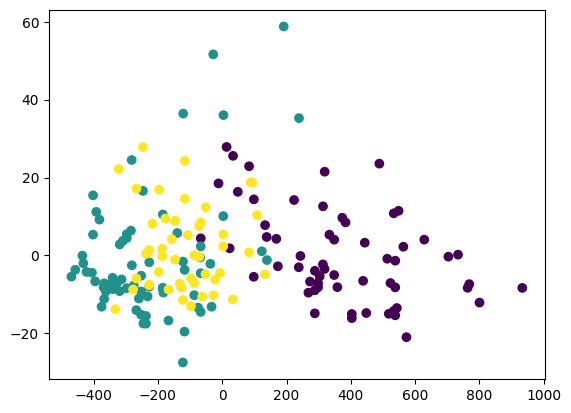
\includegraphics[width=0.8\textwidth]{output.png}
    \caption{Graph showing class separability}
\end{figure}


\newpage
\subsection{Exercise c)}

\begin{itemize}
    \item For K-Means: 
    \[
    s = 0.5722554756855064
    \]
    
    \item For EM-Clustering: 
    \[
    s = 0.26233330799498905
    \]
\end{itemize}

The k\_means is still the better algorithm, because the silhouette is greater. Silhouette values vary due to random initialization in k\_means and EM-clustering, data structure and dimensionality reduction with PCA.

\begin{figure}[h]
    \centering
    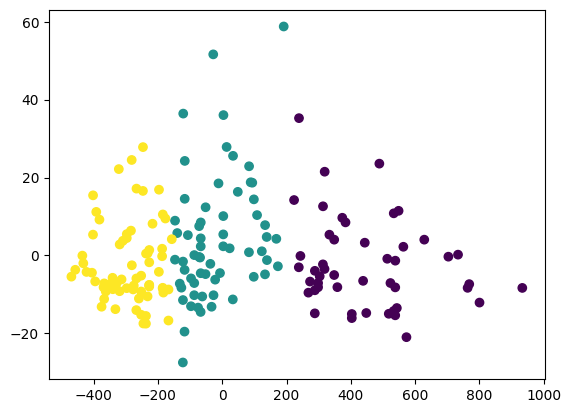
\includegraphics[width=0.8\textwidth]{output1.png}
    \caption{K-Means clustering result}
\end{figure}

\begin{figure}[h]
    \centering
    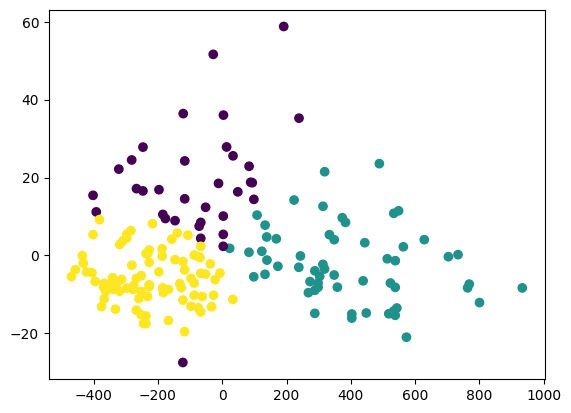
\includegraphics[width=0.8\textwidth]{output2.png}
    \caption{EM-Clustering result}
\end{figure}

\newpage
\subsection{Exercise d)}

\begin{itemize}
    \item For K-Means: 
    \[
    s = 0.6972646156059464
    \]
    
    \item For EM-Clustering: 
    \[
    s = 0.5315172918032405
    \]
\end{itemize}

The silhouette is bigger k\_means, so k\_means is still the best one.

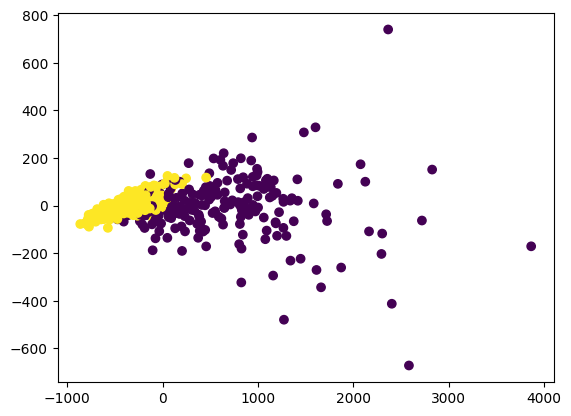
\includegraphics[width=0.8\textwidth]{output3.png}\\[1ex]

By comparating the ilhouette difference in both algorithms we would expect the same-class points to be closer to each other, which happens as we can see in the graph above.

\end{document}
